\documentclass{article}

% Language setting
% Replace `english' with e.g. `spanish' to change the document language
% \usepackage{CJKutf8}
\usepackage[english]{babel}
% \usepackage{fontspec}
% \setmainfont[Mapping=tex-text]{Kaiti SC}

% Set page size and margins
% Replace `letterpaper' with `a4paper' for UK/EU standard size
\usepackage[a4paper,top=2cm,bottom=2cm,left=3cm,right=3cm,marginparwidth=1.75cm]{geometry}

% Useful packages
\usepackage{amsmath}
\usepackage{amssymb}
\usepackage{enumitem}
\usepackage{multirow}
\usepackage{graphicx}
\usepackage{caption}
\usepackage{subcaption}
\usepackage[colorlinks=true, allcolors=blue]{hyperref}

\title{\textbf{Genetic Algorithms Assignment 1}}
\author{R11921038 Tu-Chin Chiang}

\begin{document}
% \begin{CJK*}{UTF8}{bsmi}
      
\maketitle

% \begin{abstract}
% Your abstract.
% \end{abstract}


\section{Trap Function}

Let’s check how often deception occurs in a random function.

% \vspace{1em}

\begin{enumerate}[label=(\alph*)]
      % \parindent=0em
      \item 
      Consider the case with two genes. 
      By assigning fitness values for $f(00), f(01), f(10)$, and $f(11)$, 
      does deception ever occur?

      \vspace{0.5em}

            \parindent=1em
            \textbf{No, deception never occurs.}
            The inequality (Ackley, 1985) is defined by 
            \begin{equation*}
                  \frac{a}{b} \geq \frac{2 - (\ell - z)^{-1}}{2 - z^{-1}},
            \end{equation*}
            where $a < b$, $\ell$ is the problem size, and $z$ is the number of unitation.
            The inequality is never satisfied when $\ell = 2$ and $z = 1$:
            \begin{equation*}
                  \frac{2 - (2 - 1)^{-1}}{2 - 1^{-1}} = 1 \not\leq \frac{a}{b}.
            \end{equation*}
            Therefore, deception never occurs in the case with two genes. \hfill $\square$

      \vspace{1em}

      \item
      \label{item:1b}
      Consider the case with three genes, randomly assign the fitness values 
      for $f(000)$, $f(001)$, $f(010)$, $f(011)$, $f(100)$, $f(101)$, $f(110)$, and $f(111)$ 
      with uniform distribution from 0 to 1. Repeat the experiments $10^6$ times. 
      What’s the probability that 3-deception occurs?

      \item
      Repeat (b), but with 4 genes.

            \begin{table}[h]
                  \setlength{\tabcolsep}{2em}
                  \renewcommand{\arraystretch}{1.3}
                  \centering
                  \begin{tabular}{ccc}
                        \hline
                         & $k$-deception & Probability \\
                        \hline
                        (b) & 3 & \textbf{0.005791} \\
                        (c) & 4 & \textbf{0.000286} \\
                        \hline
                  \end{tabular}
                  \caption{Probability of 3-deception and 4-deception}
            \end{table}
            \hfill $\square$



      \item
      For a problem with $ell$ genes (problem size), the probability that $k$-deception 
      does NOT occur among any $k$ genes is roughly $(1 - p)^{ell \choose k}$, 
      where $p$ is recorded in (b) and (c). 
      What’s the problem size that makes 3-deception occur with probably 0.5? 
      What’s that for 4-deception? 
      When does 3-deception occur more often than 4-deception or the other way around?


            \begin{table}[h]
                  \setlength{\tabcolsep}{1.8em}
                  \renewcommand{\arraystretch}{1.3}
                  \centering
                  \begin{tabular}{ccc}
                        \hline
                         & Scenario & Problem size $ell$ \\
                        \hline
                        (d.1) & $Prob$(3-deception) $> 0.5$ & $ell \ge \textbf{10}$ \\
                        (d.2) & $Prob$(4-deception) $> 0.5$ & $ell \ge \textbf{18}$ \\
                        \multirow{2}{*}{(d.3)} & 3-deception occurs more often & \multirow{2}{*}{$ell \le \textbf{84}$} \\
                         & than 4-deception &  \\
                        \hline
                  \end{tabular}
                  \caption{Problem size for the occurrence of different scenarios}
            \end{table}

            \parindent=0em
            (d.1)
            \begin{equation*}
            \begin{aligned}
                  1 - (1 - p)^{ell \choose 3} &= 0.5 \\
                  \Rightarrow (1- 0.005791)^{ell \choose 3} &= 0.5 \\
                  \Rightarrow {ell \choose 3} \times \log(0.994209) &= \log(0.5) \\
                  \Rightarrow {ell \choose 3} &= \frac{ell(ell-1)(ell-2)}{6} = \frac{\log(0.5)}{\log(0.994209)} = 119.36763 \\
                  \Rightarrow ell &= 9.98429, -3.49215 \pm 7.71619i \\
            \end{aligned}
            \end{equation*}

            (d.2)
            \begin{equation*}
            \begin{aligned}
                  1 - (1 - p)^{ell \choose 4} &= 0.5 \\
                  \Rightarrow (1- 0.000286)^{ell \choose 4} &= 0.5 \\
                  \Rightarrow {ell \choose 4} \times \log(0.999714) &= \log(0.5) \\
                  \Rightarrow {ell \choose 4} &= \frac{ell(ell-1)(ell-2)(ell-3)}{24} = \frac{\log(0.5)}{\log(0.999714)} = 2423.24495 \\
                  \Rightarrow ell &= 17.0696, -14.0696, 1.5 \pm 15.4891i \\
            \end{aligned}
            \end{equation*}

            (d.3)
            \begin{equation*}
            \begin{aligned}
                  1 - (1 - p_3)^{ell \choose 3} &> 1 - (1 - p_4)^{ell \choose 4} \\
                  \Rightarrow {ell \choose 3} \times \log(1 - 0.005791) &< {ell \choose 4} \times \log(1 - 0.000286) \\
                  \Rightarrow ell - 3 &< 4 \times \frac{\log(1 - 0.005791)}{\log(1 - 0.000286)} \\
                  \Rightarrow ell &< 84.2027 \\
            \end{aligned}
            \end{equation*}

            \vspace{1.5em}
            \parindent=1em
            In summary, the problem size at which 3-deception is likely to occur with a probability of 0.5 is $ell \geq 10$, 
            while for 4-deception, it is $ell \geq 18$. When the problem size is less than 84, 
            3-deception occurs more frequently than 4-deception. 
            This is attributed to the fact that the combinations of genes for 4-deception increase more rapidly as the problem size grows.
            
            \begin{figure}[ht]
                  \centering
                  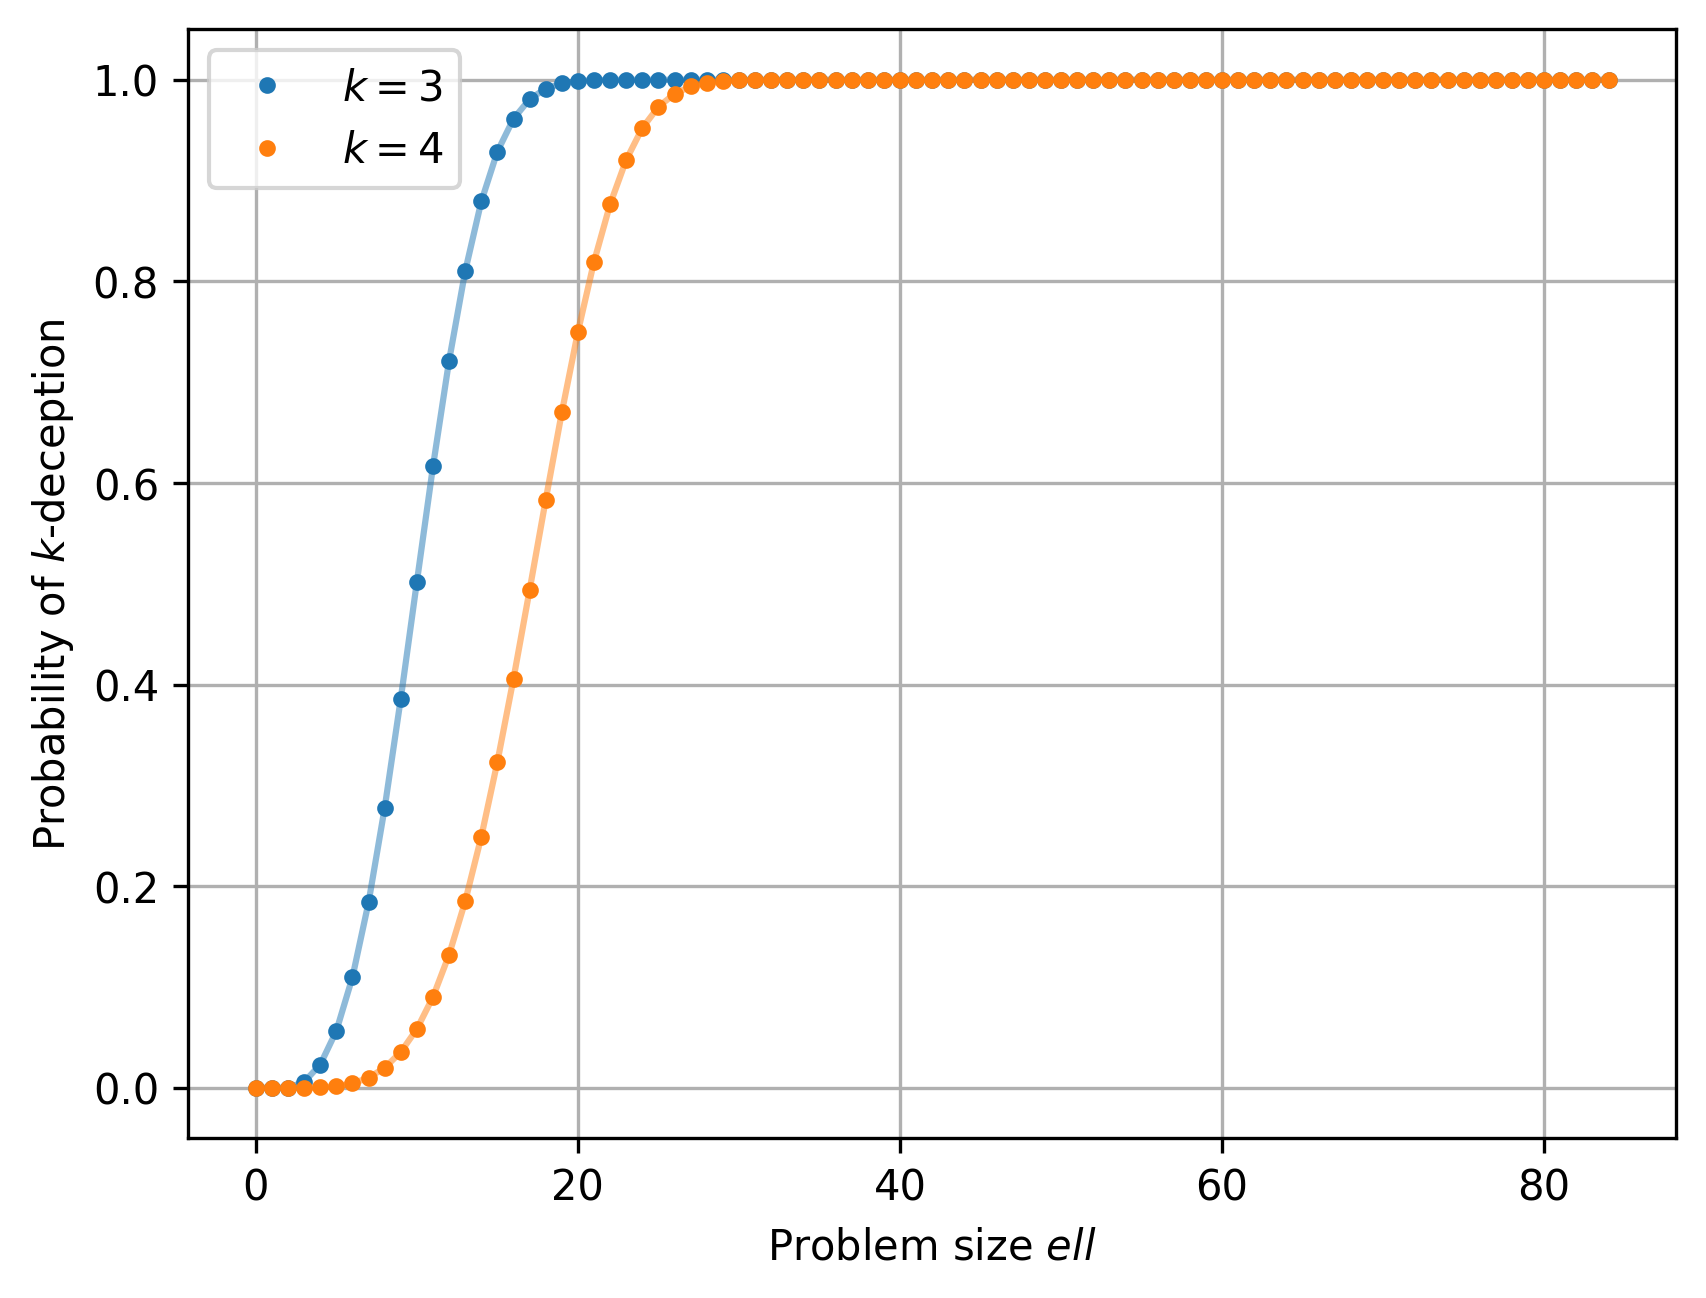
\includegraphics[width=0.7\linewidth]{fig-deception.png}
                  \caption{Probabilities of 3 and 4-deception}
                  \label{fig:deception_prob}
            \end{figure}

            However, a concern arises when examining the probabilities of 3 and 4-deception, particularly 
            as the problem size becomes larger, as illustrated in Figure~\ref{fig:deception_prob}. 
            The probabilities of both 3 and 4-deception approach 1 when the problem size is large, with probabilities greater 
            than 0.999 observed at problem sizes of 21 and 30, respectively. 
            Therefore, despite the maximum problem size at which 3-deception occurs more often being 84, the results indicate that 
            both 3 and 4-deception occur with high probabilities when the problem size reaches 84.
            

            \hfill $\square$

\end{enumerate}

% \newpage
\vspace{5em}
\section{Convergence Time}
Thierens’ convergence-time model assumes perfect mixing. Verify the model
with (1) one-point XO, (2) uniform XO, and (3) population-wise shuffling: the set of genes at a particular position of offspring is a random shuffle
of the set of genes at the same position of parents.
\begin{enumerate}[label=(\alph*)]
      \item 
      Experiment these three XO’s with a SGA on the OneMax problem with
      different sizes (ell) of 50, 100, 150, 200, 250, 300, 350, 400, 450, and 500. Plot
      the results on a figure with problem size versus convergence time. (repeat $=30$, population
      size $= 4\times ell \times ln(ell)$, and tournament size $=2$.)

      \begin{figure}[ht]
            \centering
            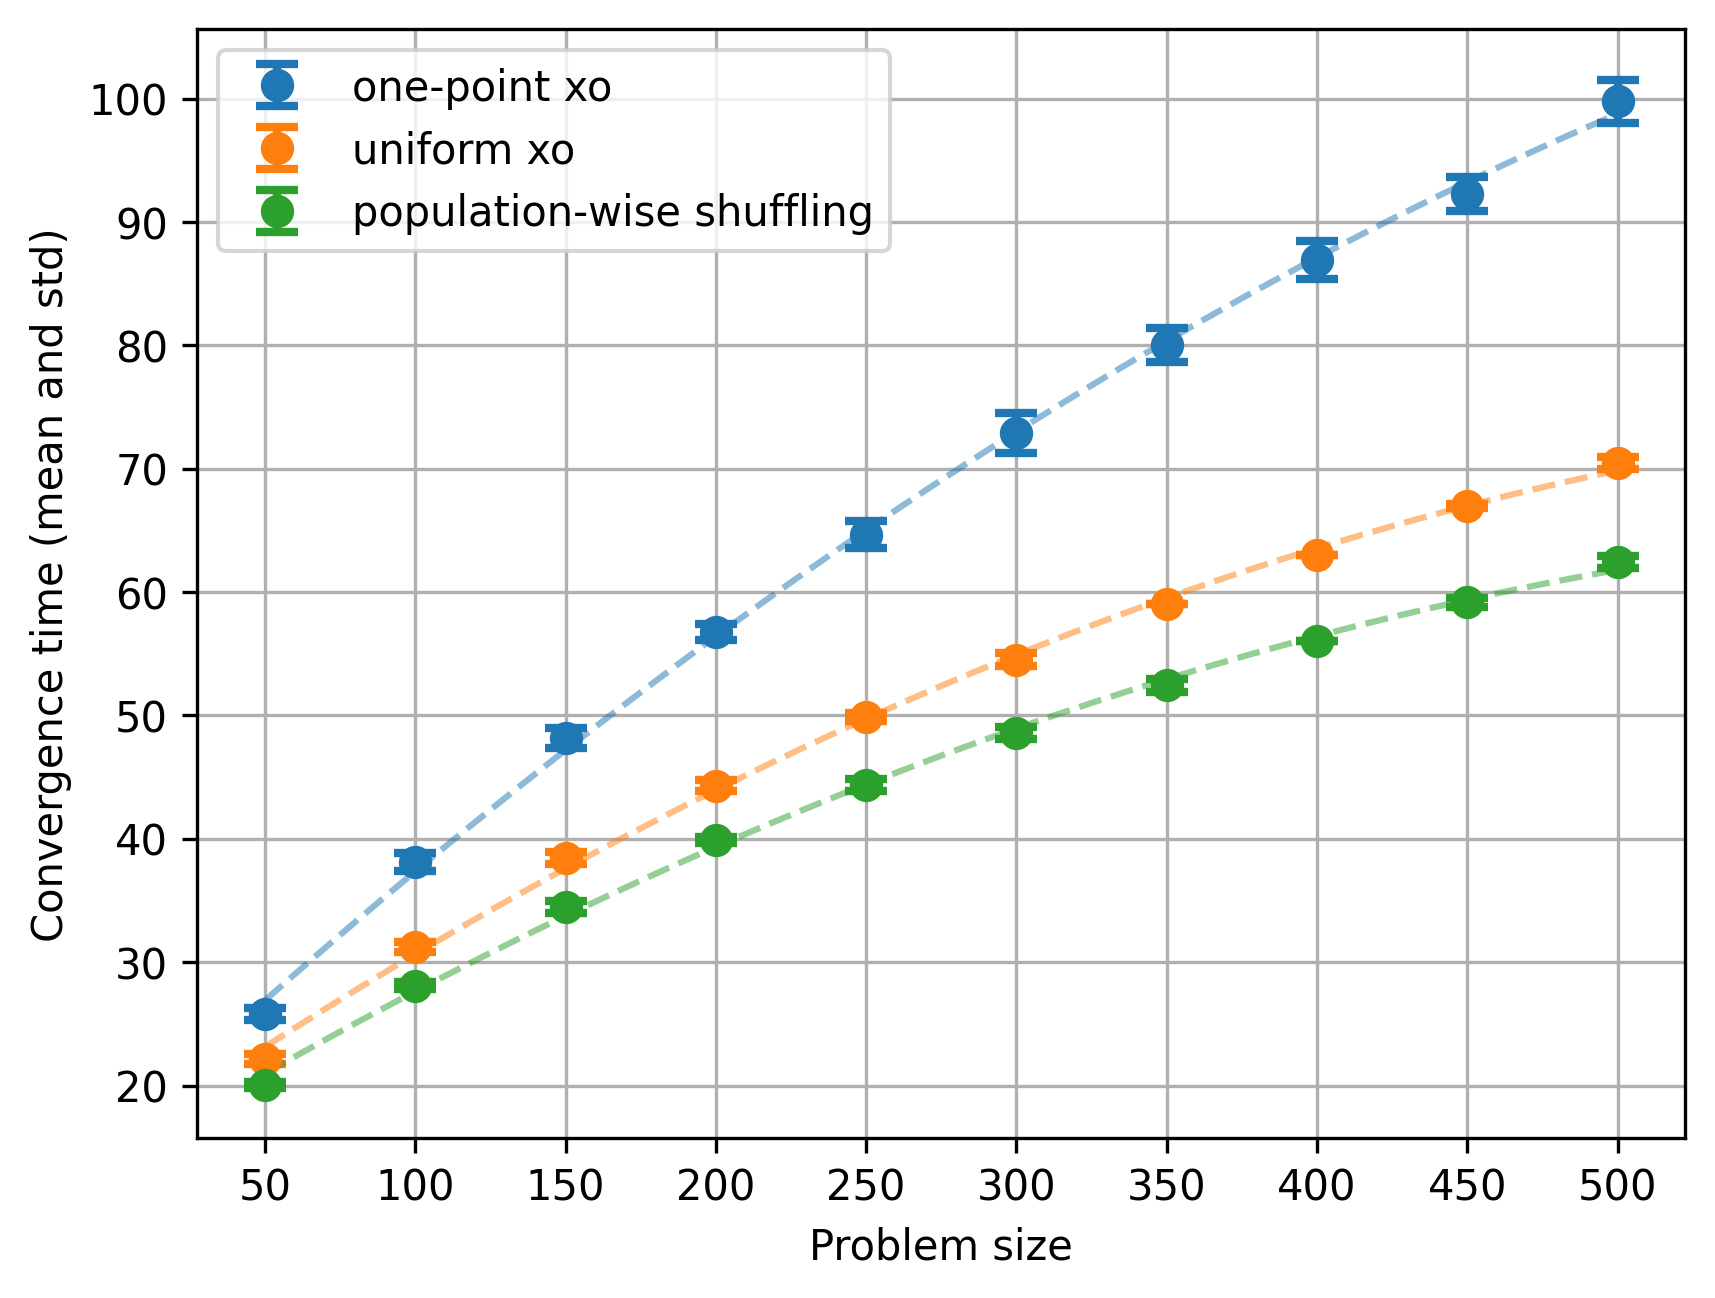
\includegraphics[width=0.7\linewidth]{fig-tconv_ell.png}
            \caption{\label{fig:convergence_time}Convergence time of different XO methods}
      \end{figure}
      \parindent=1em
      Due to the independent variables of the problem size, I plot the average convergence time versus
      the problem size of three XO methods in Figure~\ref{fig:convergence_time}. 
      The results show that the convergence time of the one-point XO is the longest, followed by the uniform XO,
      and the population-wise shuffling has the shortest convergence time under the same problem size.
      \hfill $\square$
      \vspace{0.5em}
      
      \item
      What’s the theoretical value of selection intensity? How does that compare
      with the selection intensity measured in your experiments? Is selection
      intensity really invariant with generation?

      \parindent=0em
      (b.1)
      
            \begin{equation*}
            \begin{aligned}
                  \text{Selection intensity } I &= \sqrt{2 \times \Bigl ( ln(s) - ln \bigl (\sqrt{4.14 \times ln(s)}\bigr ) \Bigr )} \\
                  &=  \sqrt{2 \times \Bigl ( ln(2) - ln \bigl (\sqrt{4.14 \times ln(2)}\bigr ) \Bigr )} \\
                  &\approx 0.576291 \\
            \end{aligned}
            \end{equation*}

      (b.2, b.3)
      
      
      \begin{figure}[ht]
            \centering
            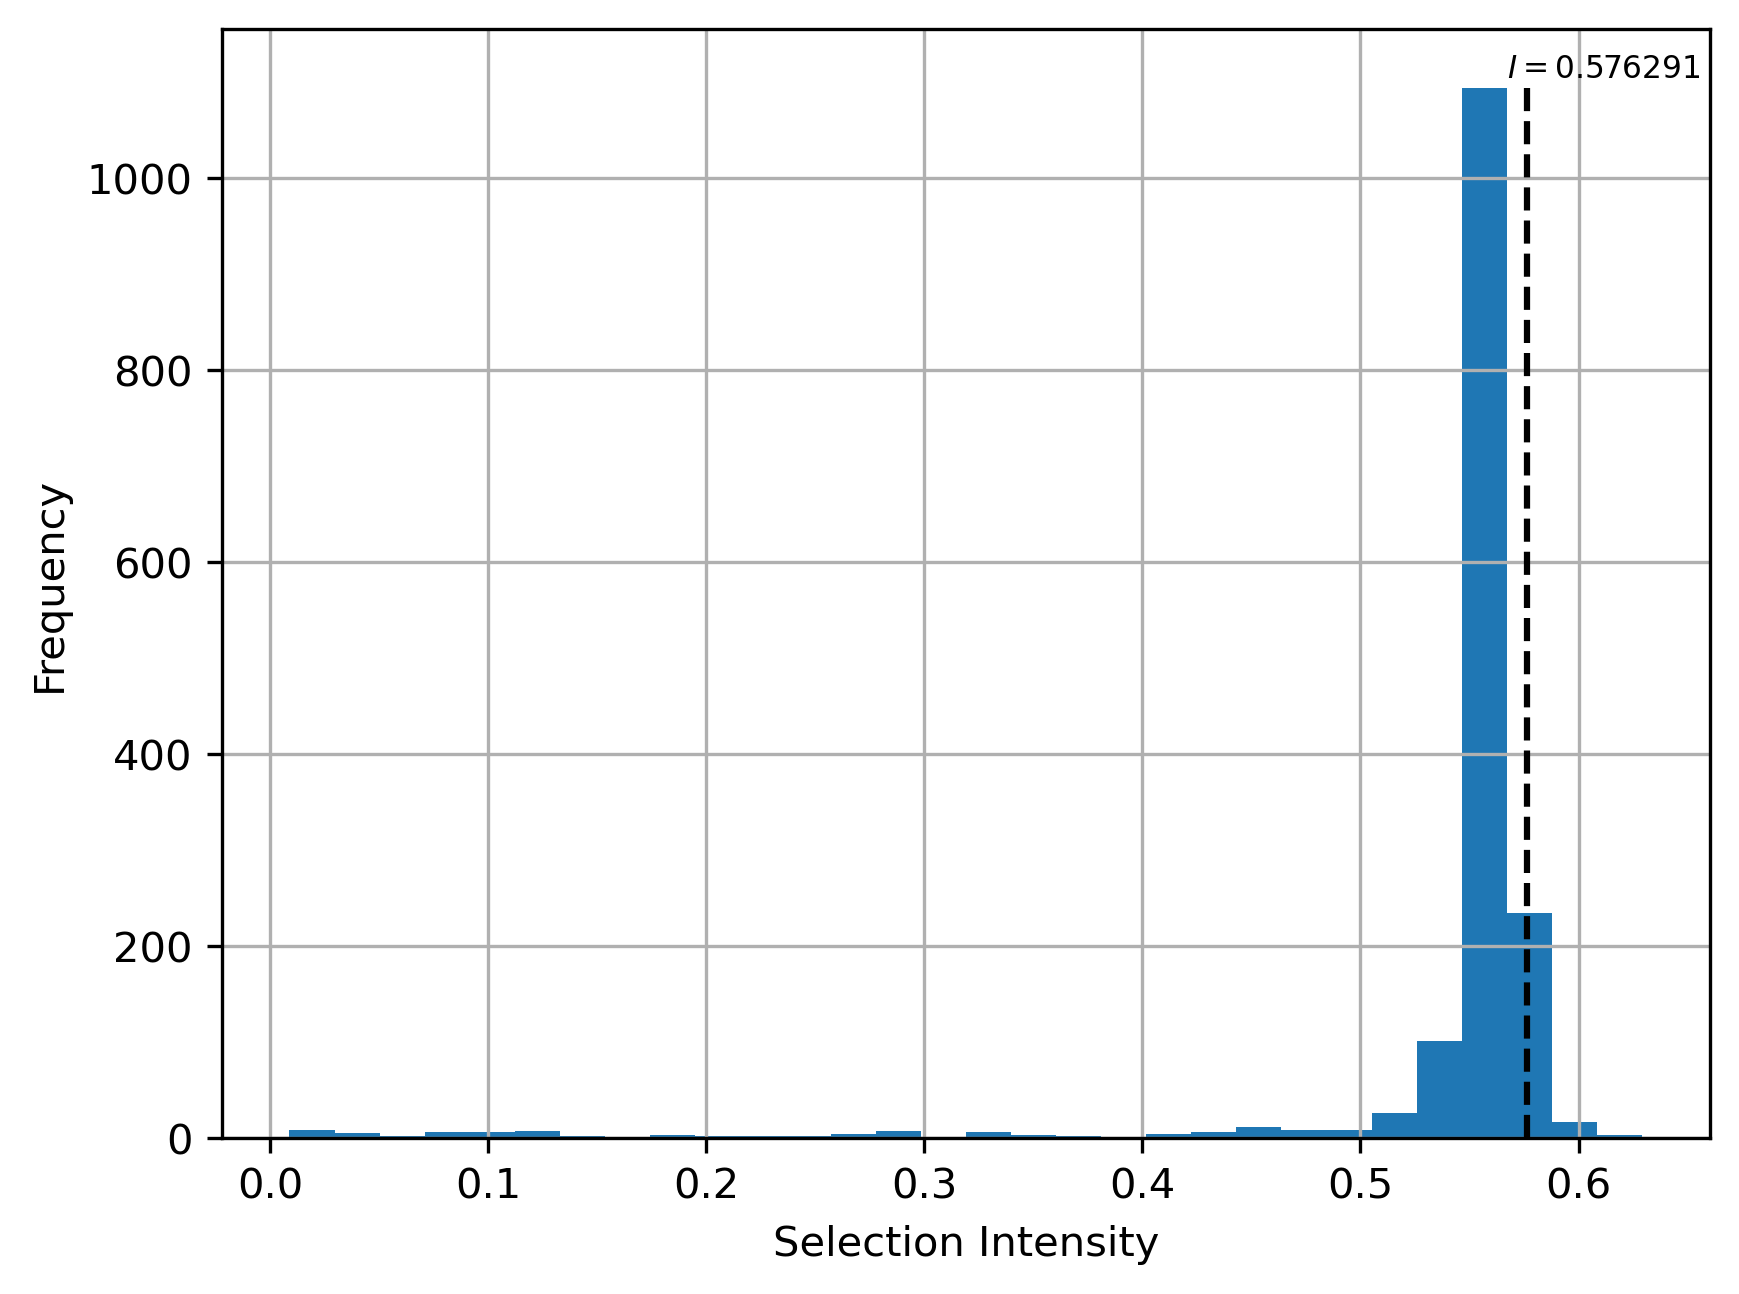
\includegraphics[width=0.7\linewidth]{fig-intensity_hist.png}
            \caption{Histograms of selection intensity}
            \label{fig:intensity}
      \end{figure}
      
            \parindent=1em
            The histogram of the selection intensities of three XO methods with 1 run is shown in 
            Figure~\ref{fig:intensity}. The results show that 68.98\% of the selection intensities of three 
            XO methods are between 0.546493 and 0.567167, which implies, on one hand, the selection intensities
            of the tournament slection are \textbf{generally invariant with generation.} 
            On the other hand, most of the selection intensities are \textbf{slightly less than the theoretical value of 0.576291}.
            
            Furthermore, a few portion of the selection intensities that are less than 0.5 occur in the last 2 to 3 generations. 
            This is likely because that the population diversity 
            decreases dramatically in the last few generations, which leads to a lower selection
            differential (\textit{i.e.}, $\bar{f}_{t+1} - \bar{f}_{t}$) and thus a lower selection intensity. \hfill $\square$

      \vspace{0.5em}

      \item
      How does Thierens’ model compare with your results?

      \begin{figure}[ht]
            \centering
            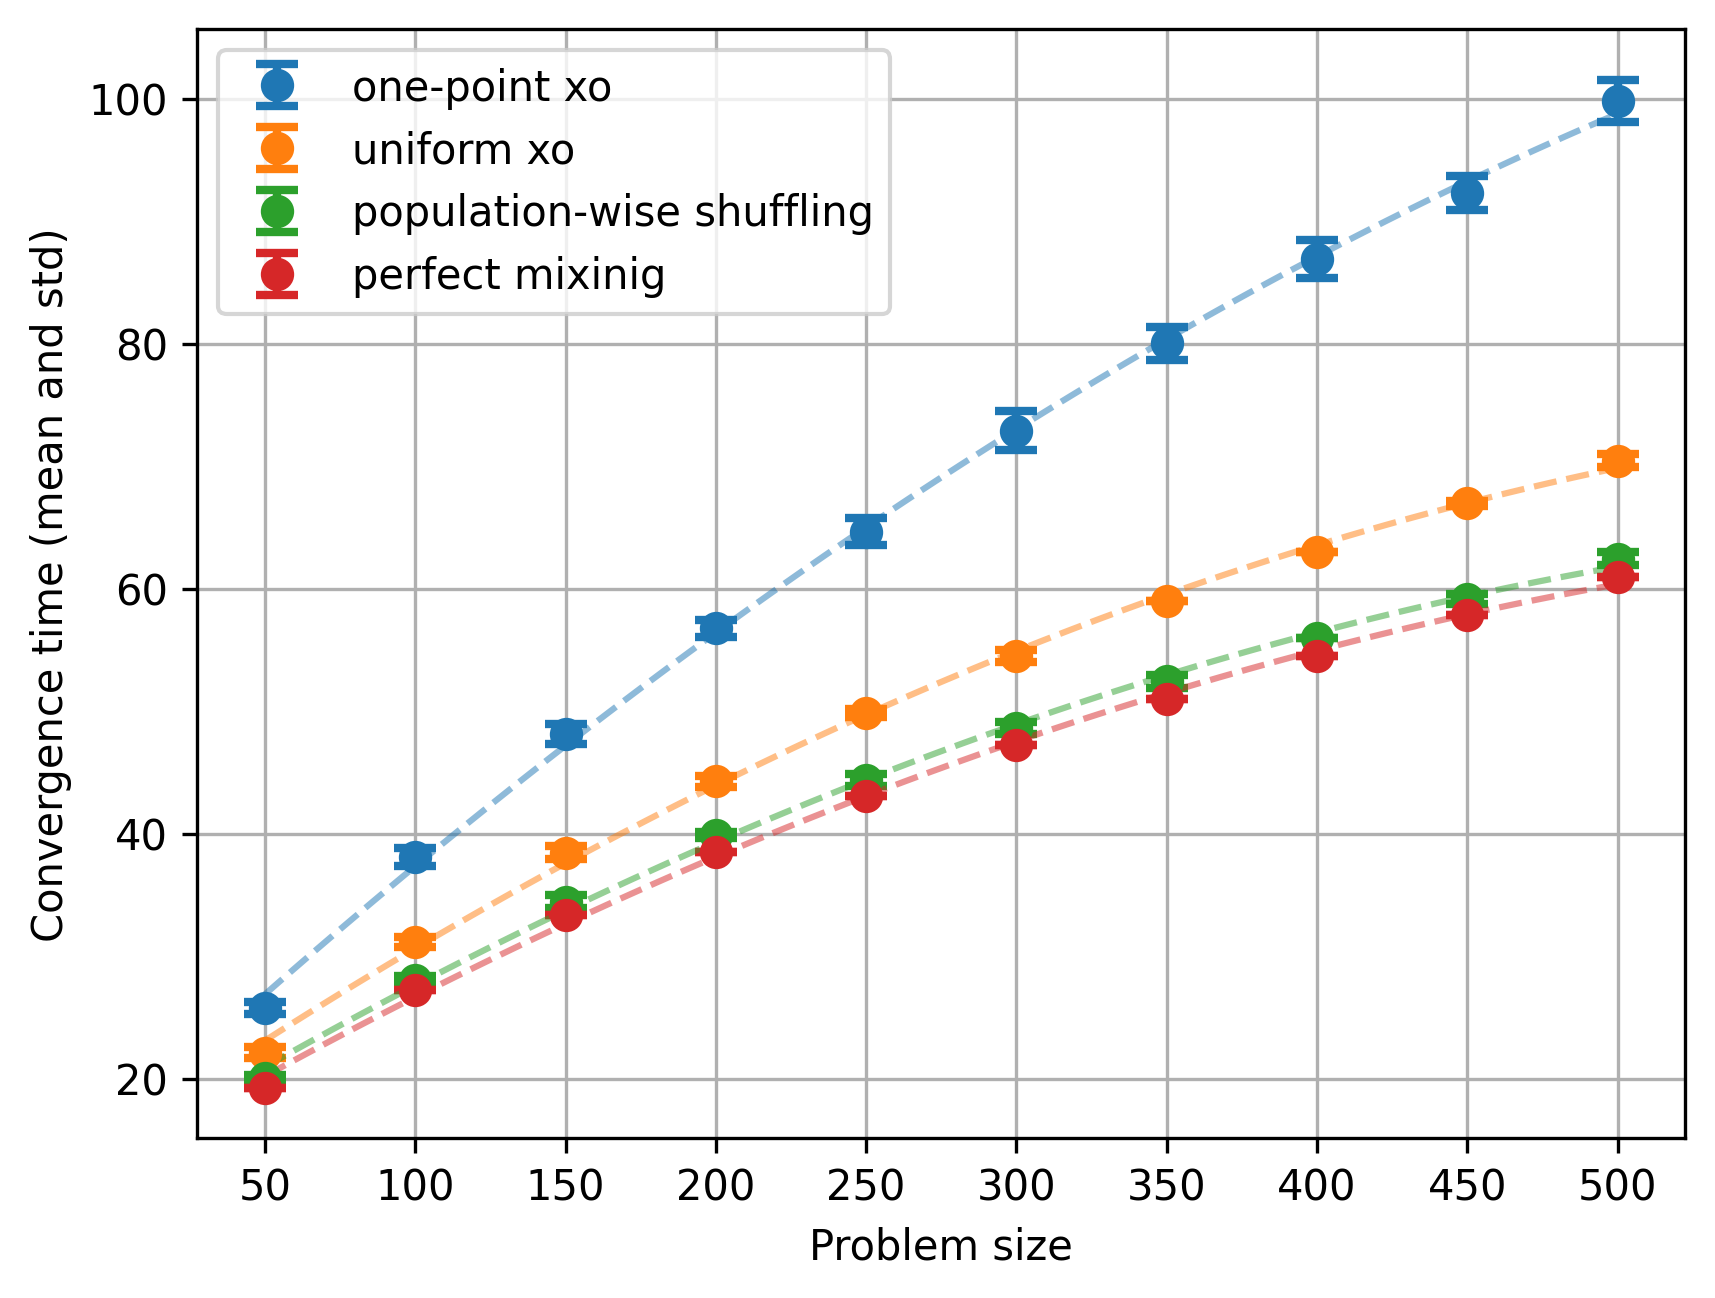
\includegraphics[width=0.7\linewidth]{fig-tconv_perfect.png}
            \caption{Convergence time of different XO methods and perfect mixing}
            \label{fig:tconv_perfect}
      \end{figure}
      
      \parindent=1em
      The main difference between Thierens' model and the experiments lies in the mixing method. 
      Thierens' model assumes perfect mixing, which employs a crossover operator that significantly disrupts the population 
      and establishes an underlying distribution of fitness. To compare the results of the three XO methods with Thierens' model, 
      we first evaluate the convergence time of the three XO methods relative to perfect mixing. 
      Then, we assess disruption by examining the uniformity and standard deviation of the fitness values within the population.
      
      The values and the trends of convergene time are illustrated in Figure~\ref{fig:tconv_perfect}.
      The convergence time of the perfect mixing is computed from the equation of Thierens' model:
      \begin{equation*}
            t_{conv} = \frac{\pi}{2} \times \frac{\sqrt{ell}}{I},
      \end{equation*}
      where $I$ is the theorectical value 0.576291 of selection intensity.
      The results show that the convergence time of the perfect mixing is the shortest for each problem size.

      \vspace{1.5em}
      
      
      \begin{figure}[h]
            \centering
            \begin{subfigure}[b]{0.32\linewidth}
                  \centering
                  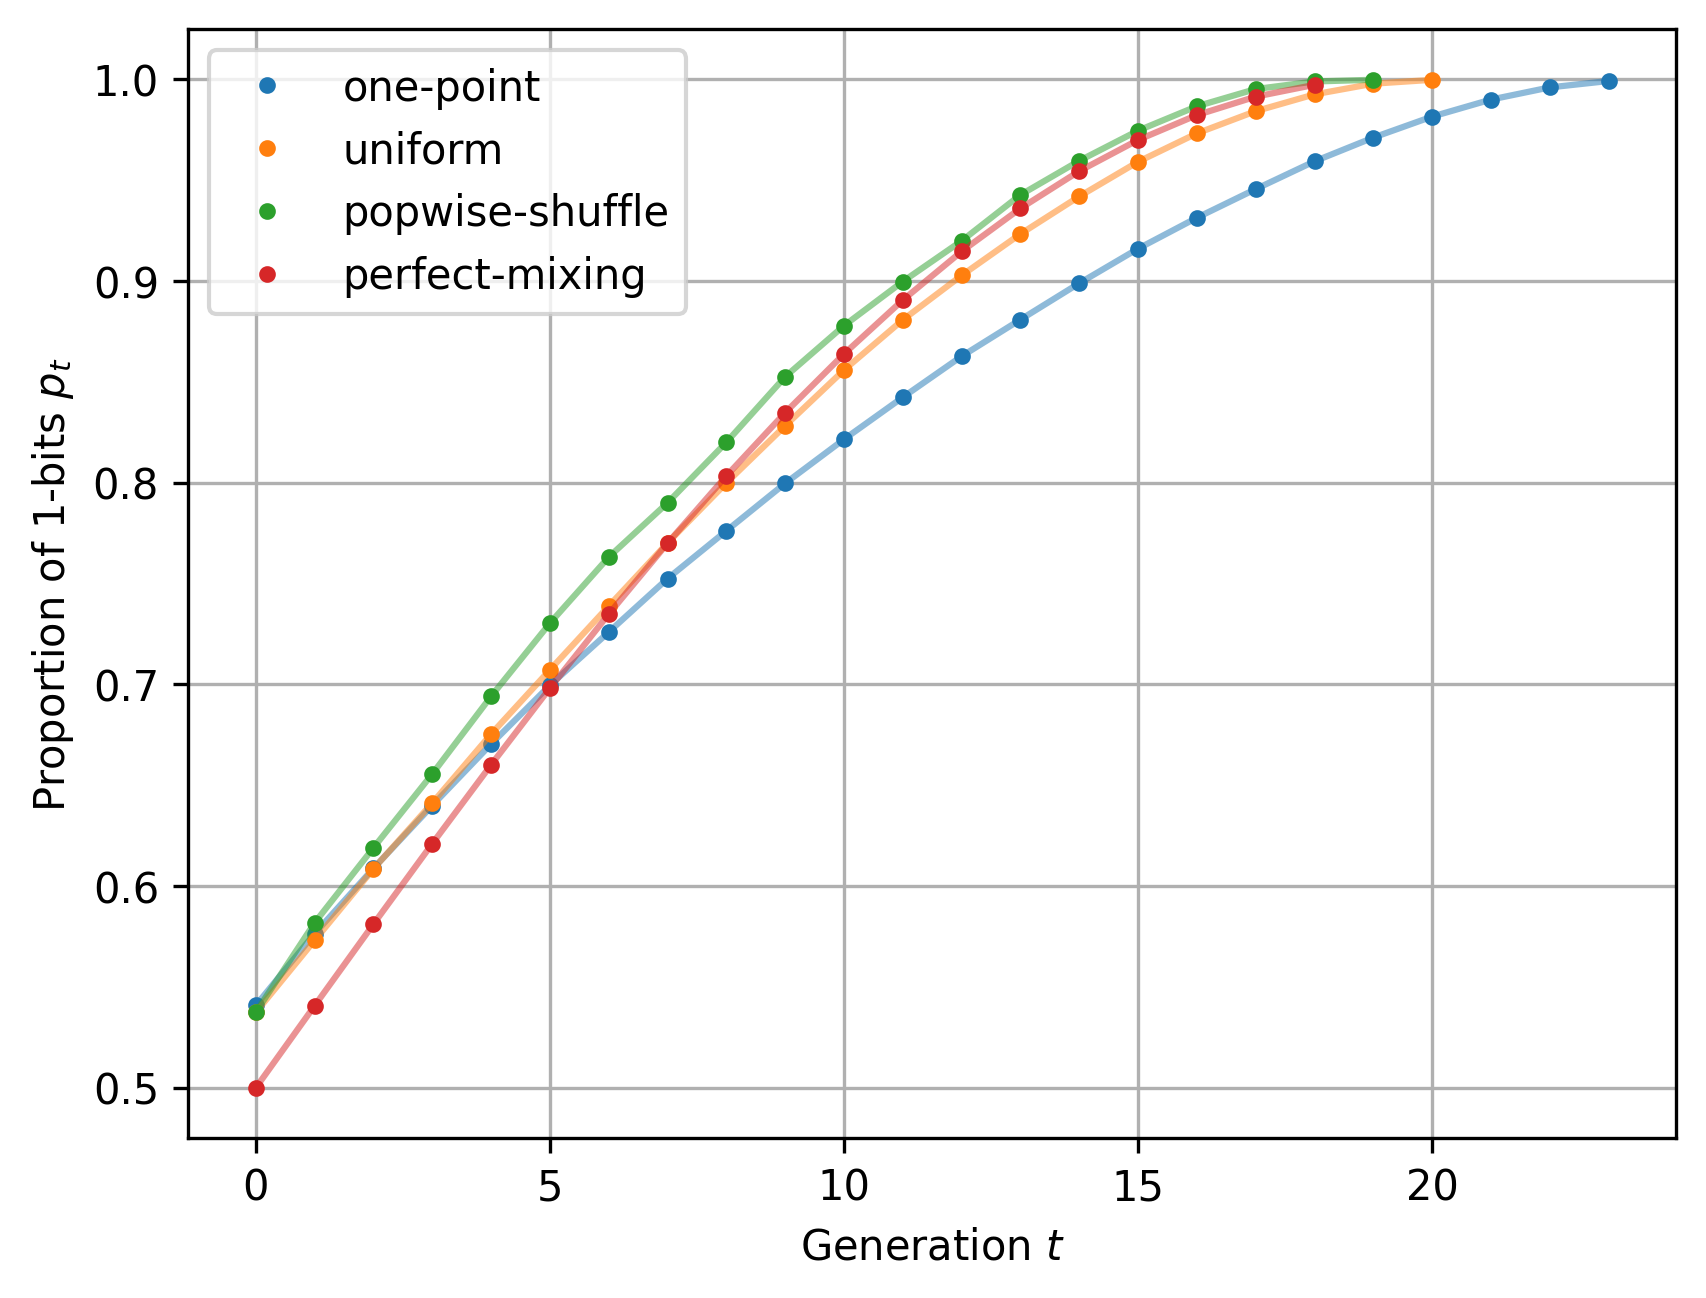
\includegraphics[width=\linewidth]{fig-uni_50.png}
                  \caption{$ell=50$}
                  \label{fig:uni-50}
            \end{subfigure}
            \hfill
            \begin{subfigure}[b]{0.32\linewidth}
                  \centering
                  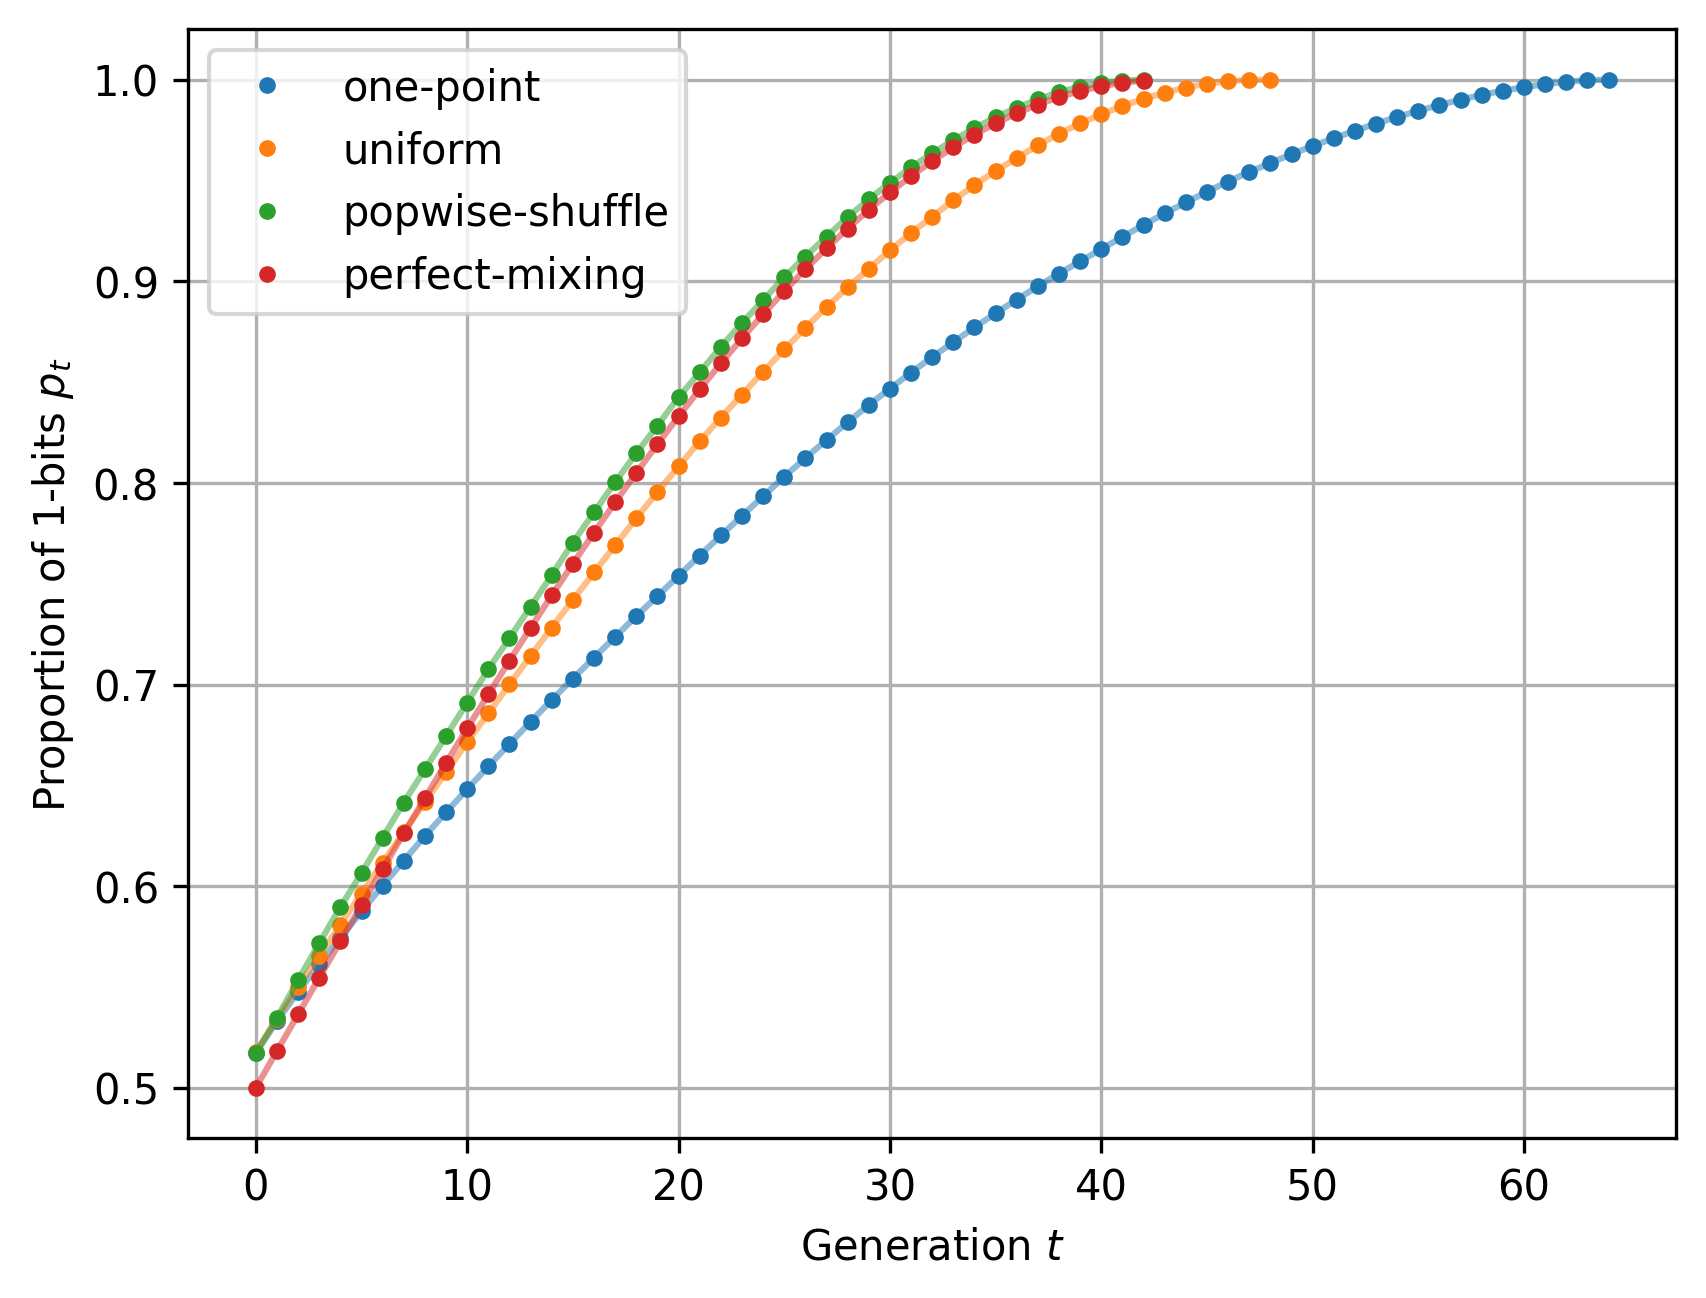
\includegraphics[width=\linewidth]{fig-uni_250.png}
                  \caption{$ell=250$}
                  \label{fig:uni-250}
            \end{subfigure}
            \hfill
            \begin{subfigure}[b]{0.32\linewidth}
                  \centering
                  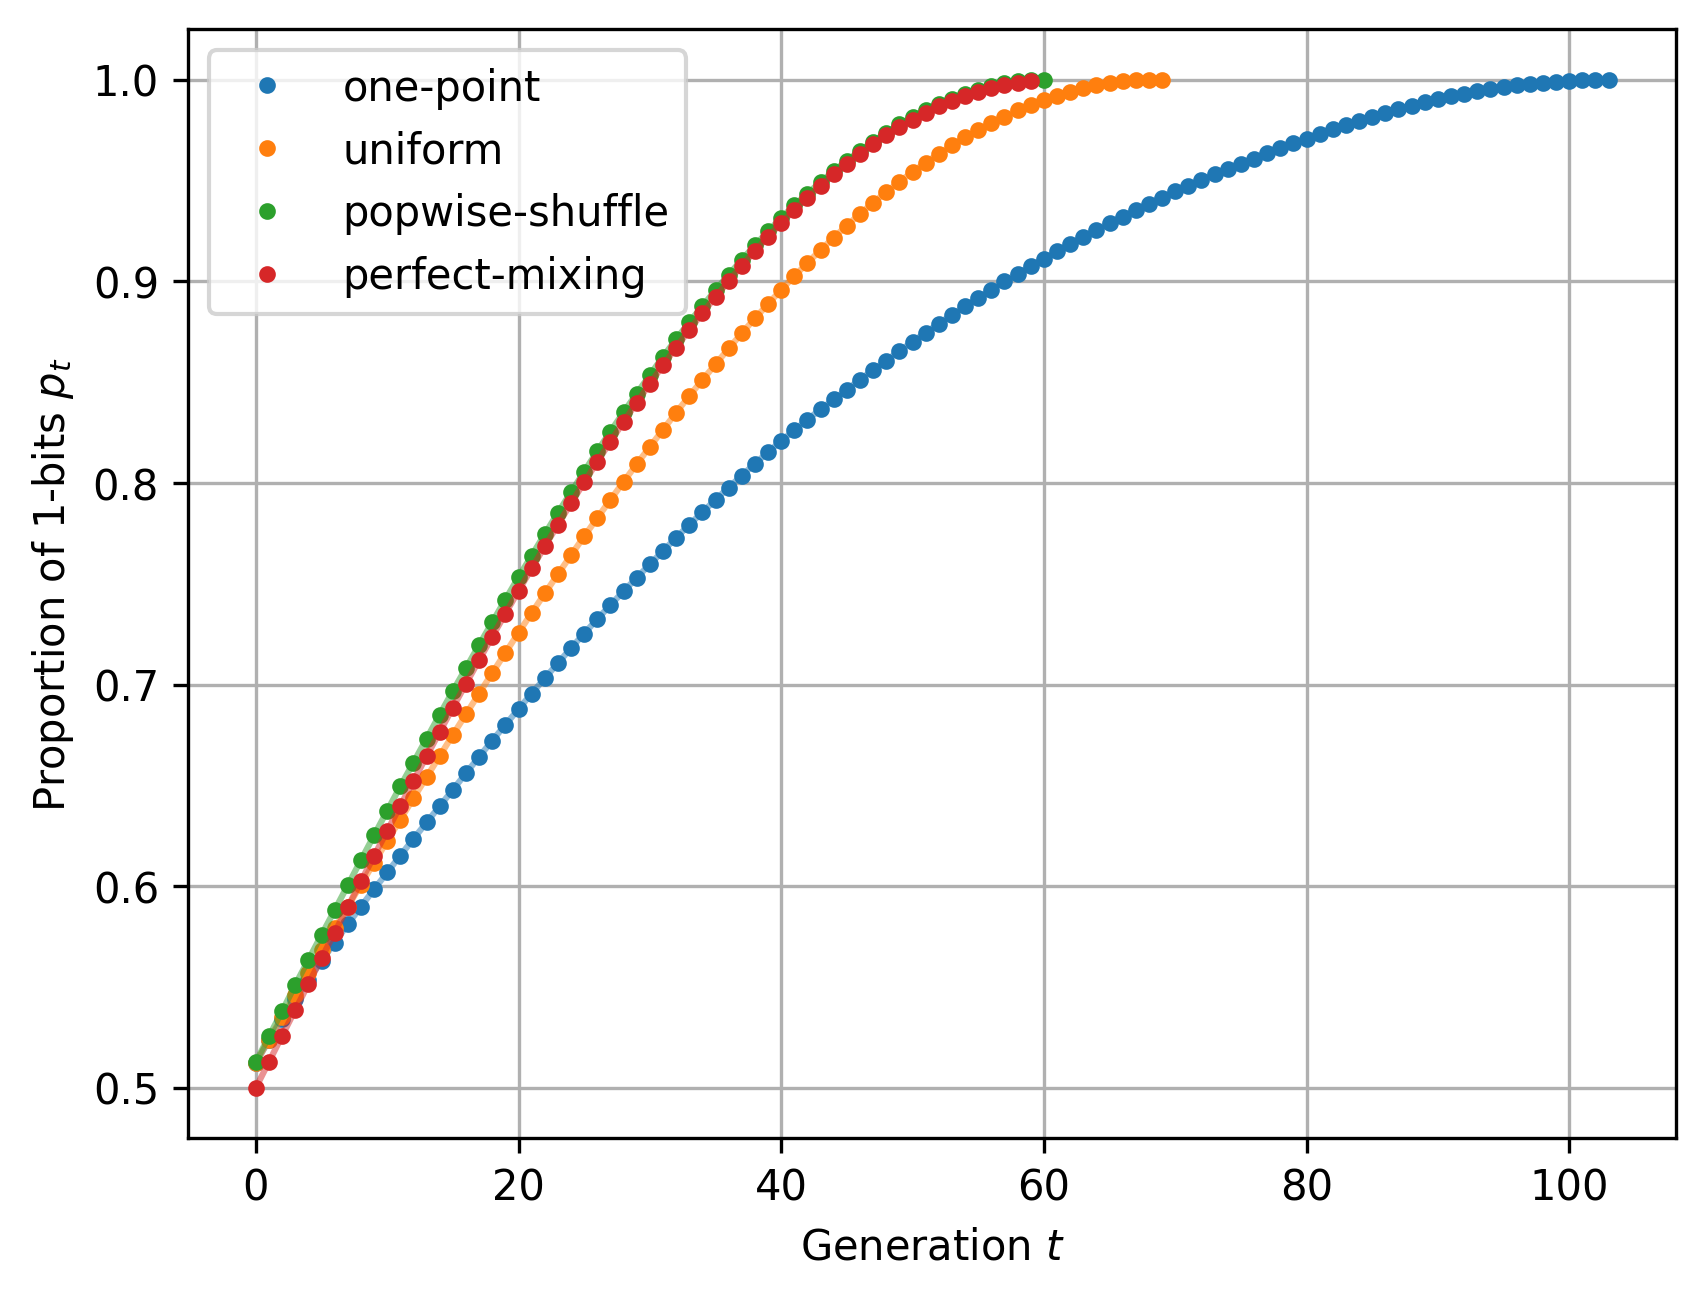
\includegraphics[width=\linewidth]{fig-uni_500.png}
                  \caption{$ell=500$}
                  \label{fig:uni-500}
            \end{subfigure}
            \caption{Unitation of different XO methods}
            \label{fig:unitation}
      \end{figure}
      
      \begin{figure}[h]
            \centering
            \begin{subfigure}[b]{0.32\linewidth}
                  \centering
                  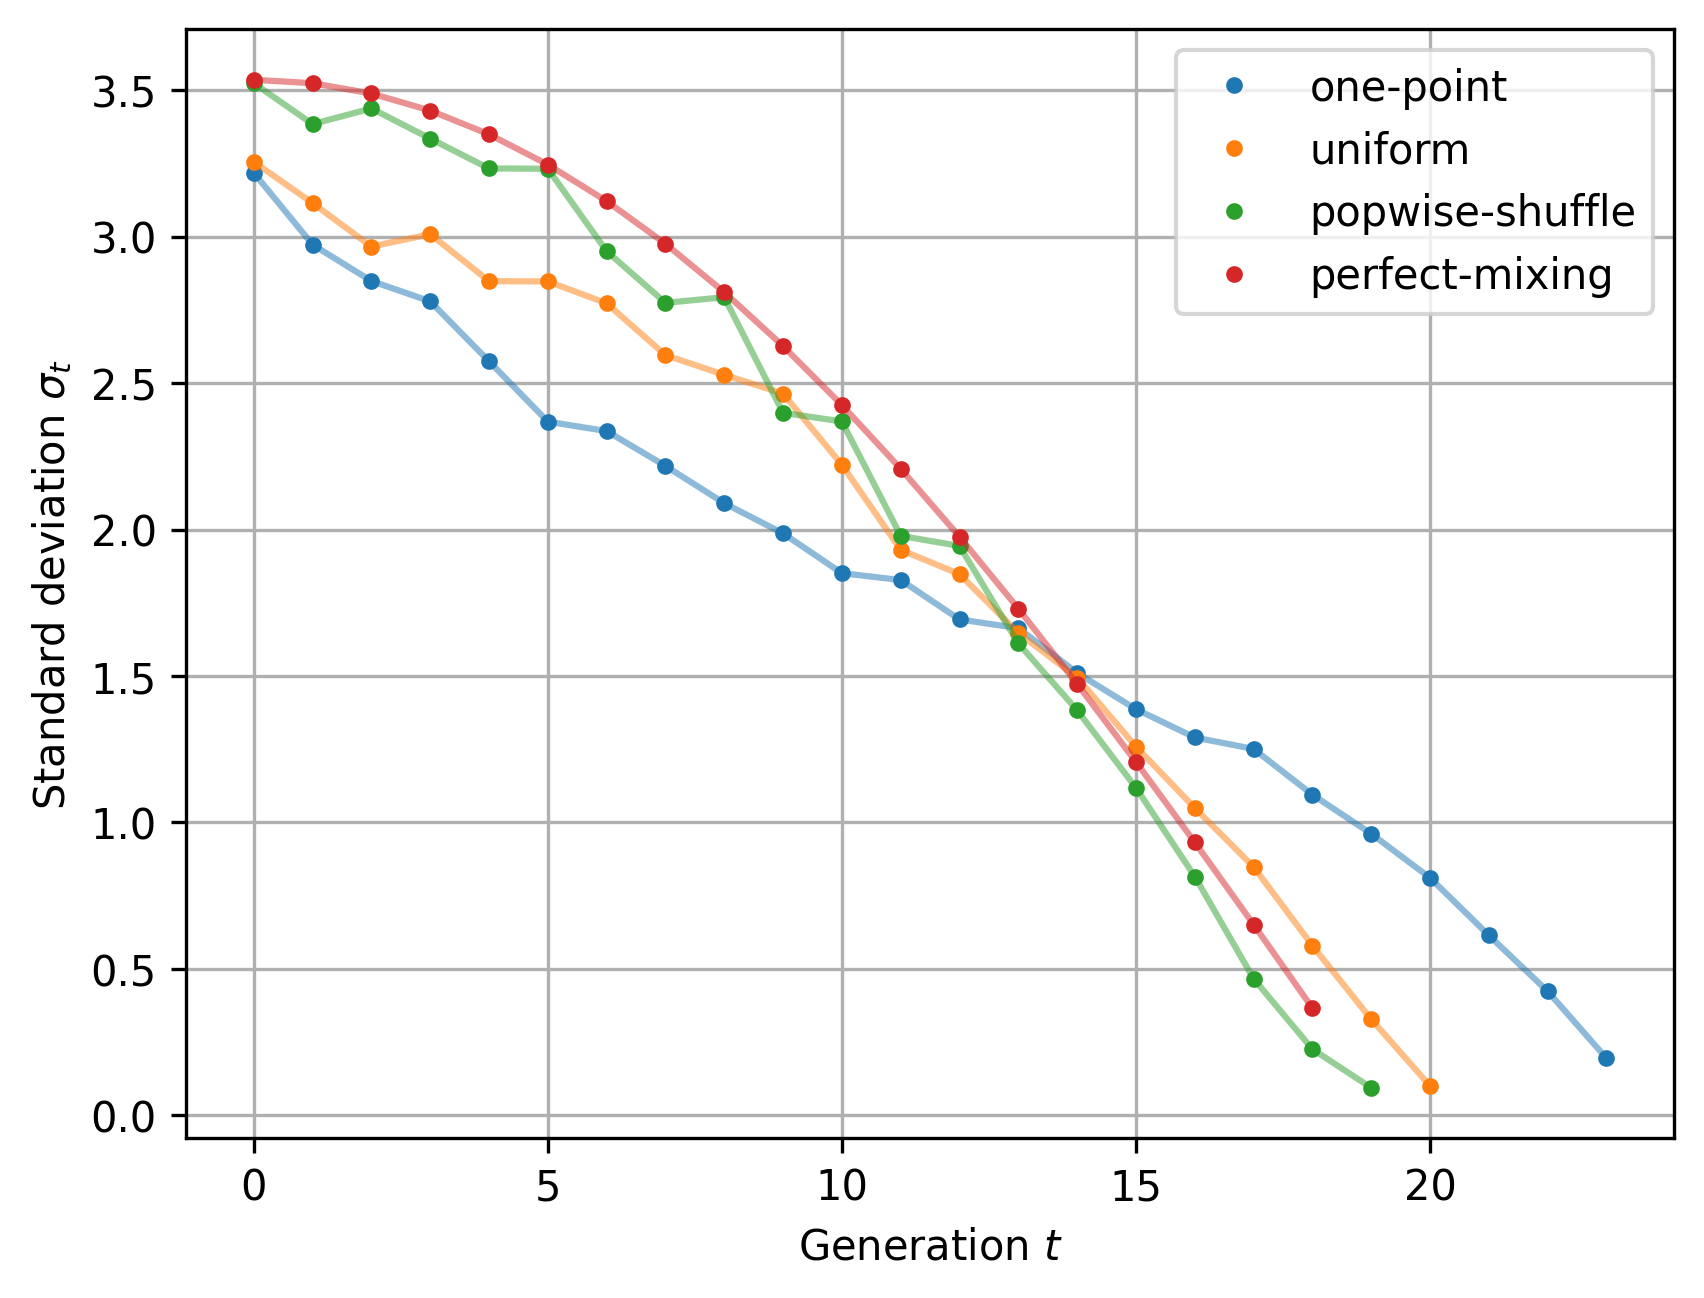
\includegraphics[width=\linewidth]{fig-std_50.png}
                  \caption{$ell=50$}
                  \label{fig:std-50}
            \end{subfigure}
            \hfill
            \begin{subfigure}[b]{0.32\linewidth}
                  \centering
                  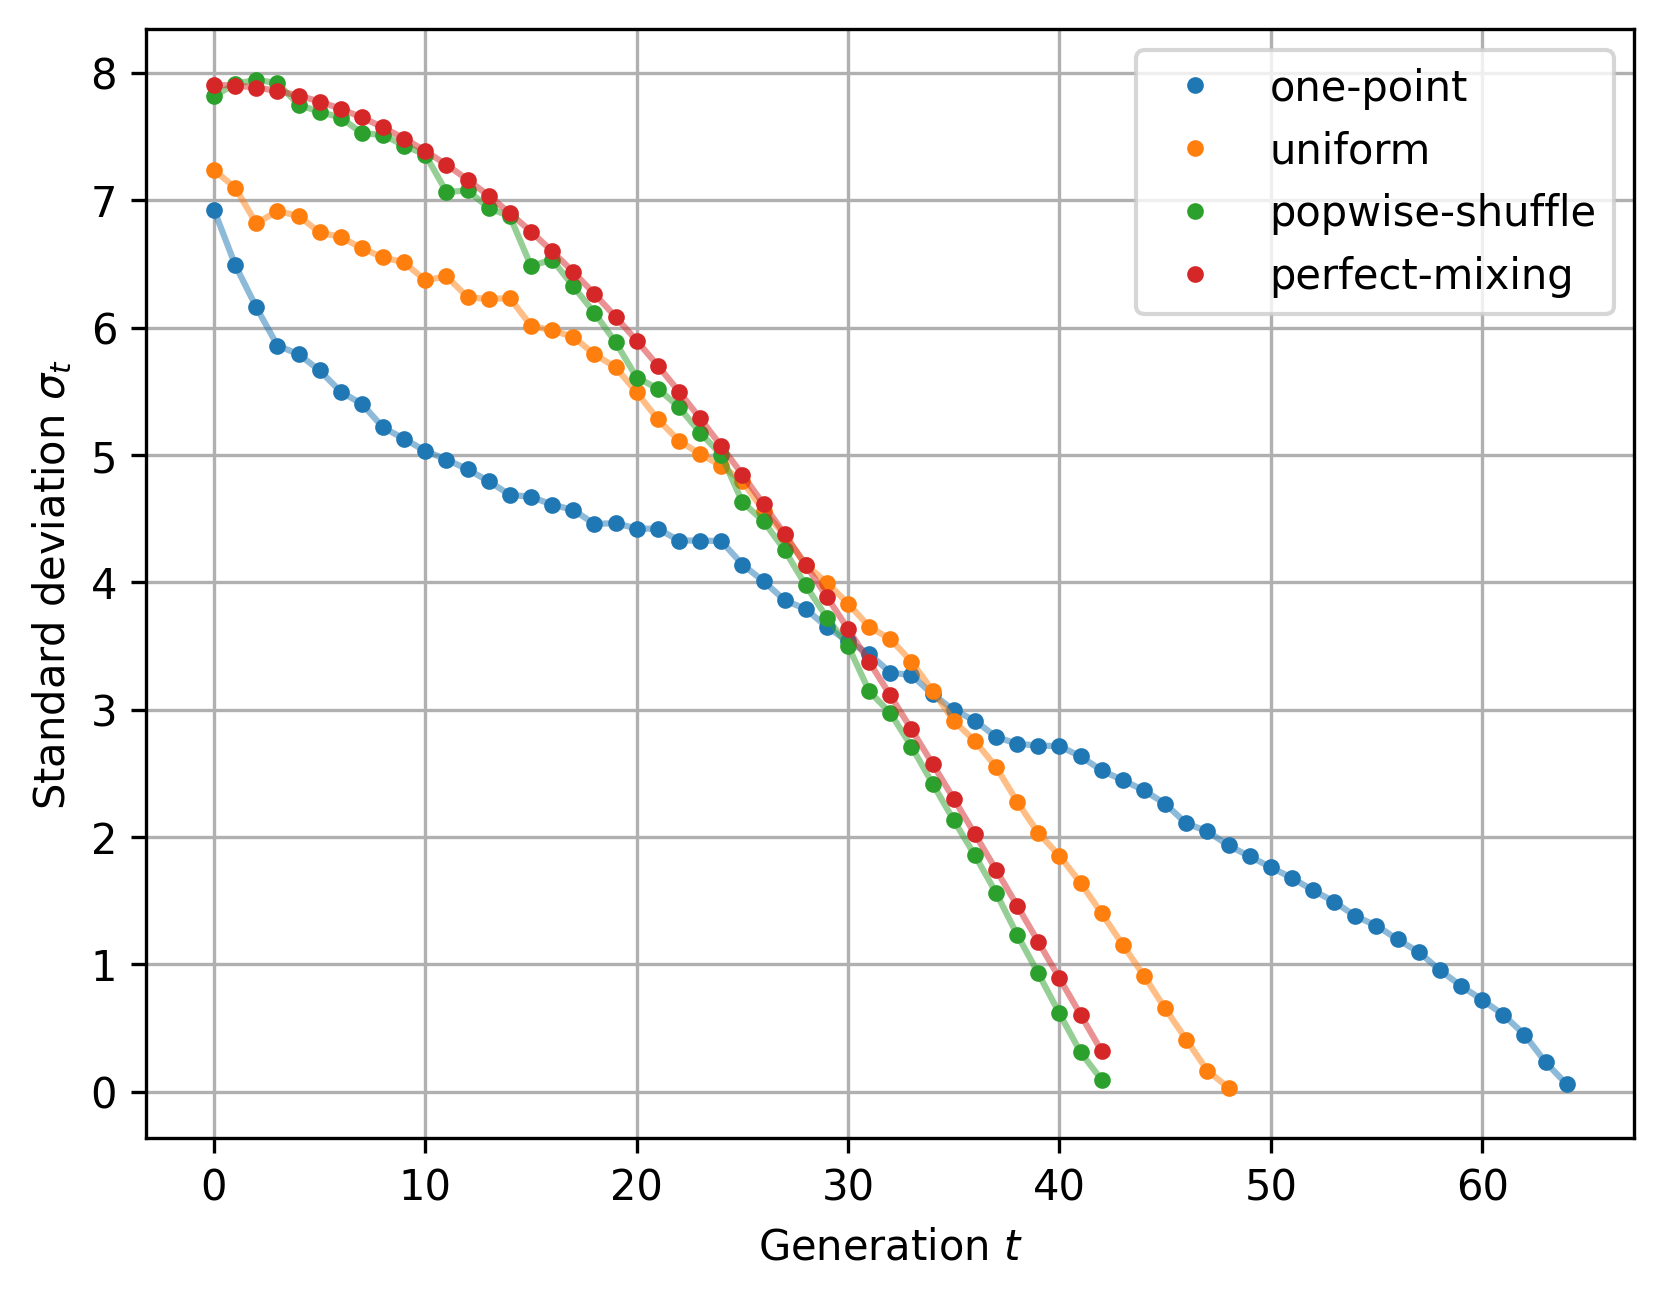
\includegraphics[width=\linewidth]{fig-std_250.png}
                  \caption{$ell=250$}
                  \label{fig:std-250}
            \end{subfigure}
            \hfill
            \begin{subfigure}[b]{0.32\linewidth}
                  \centering
                  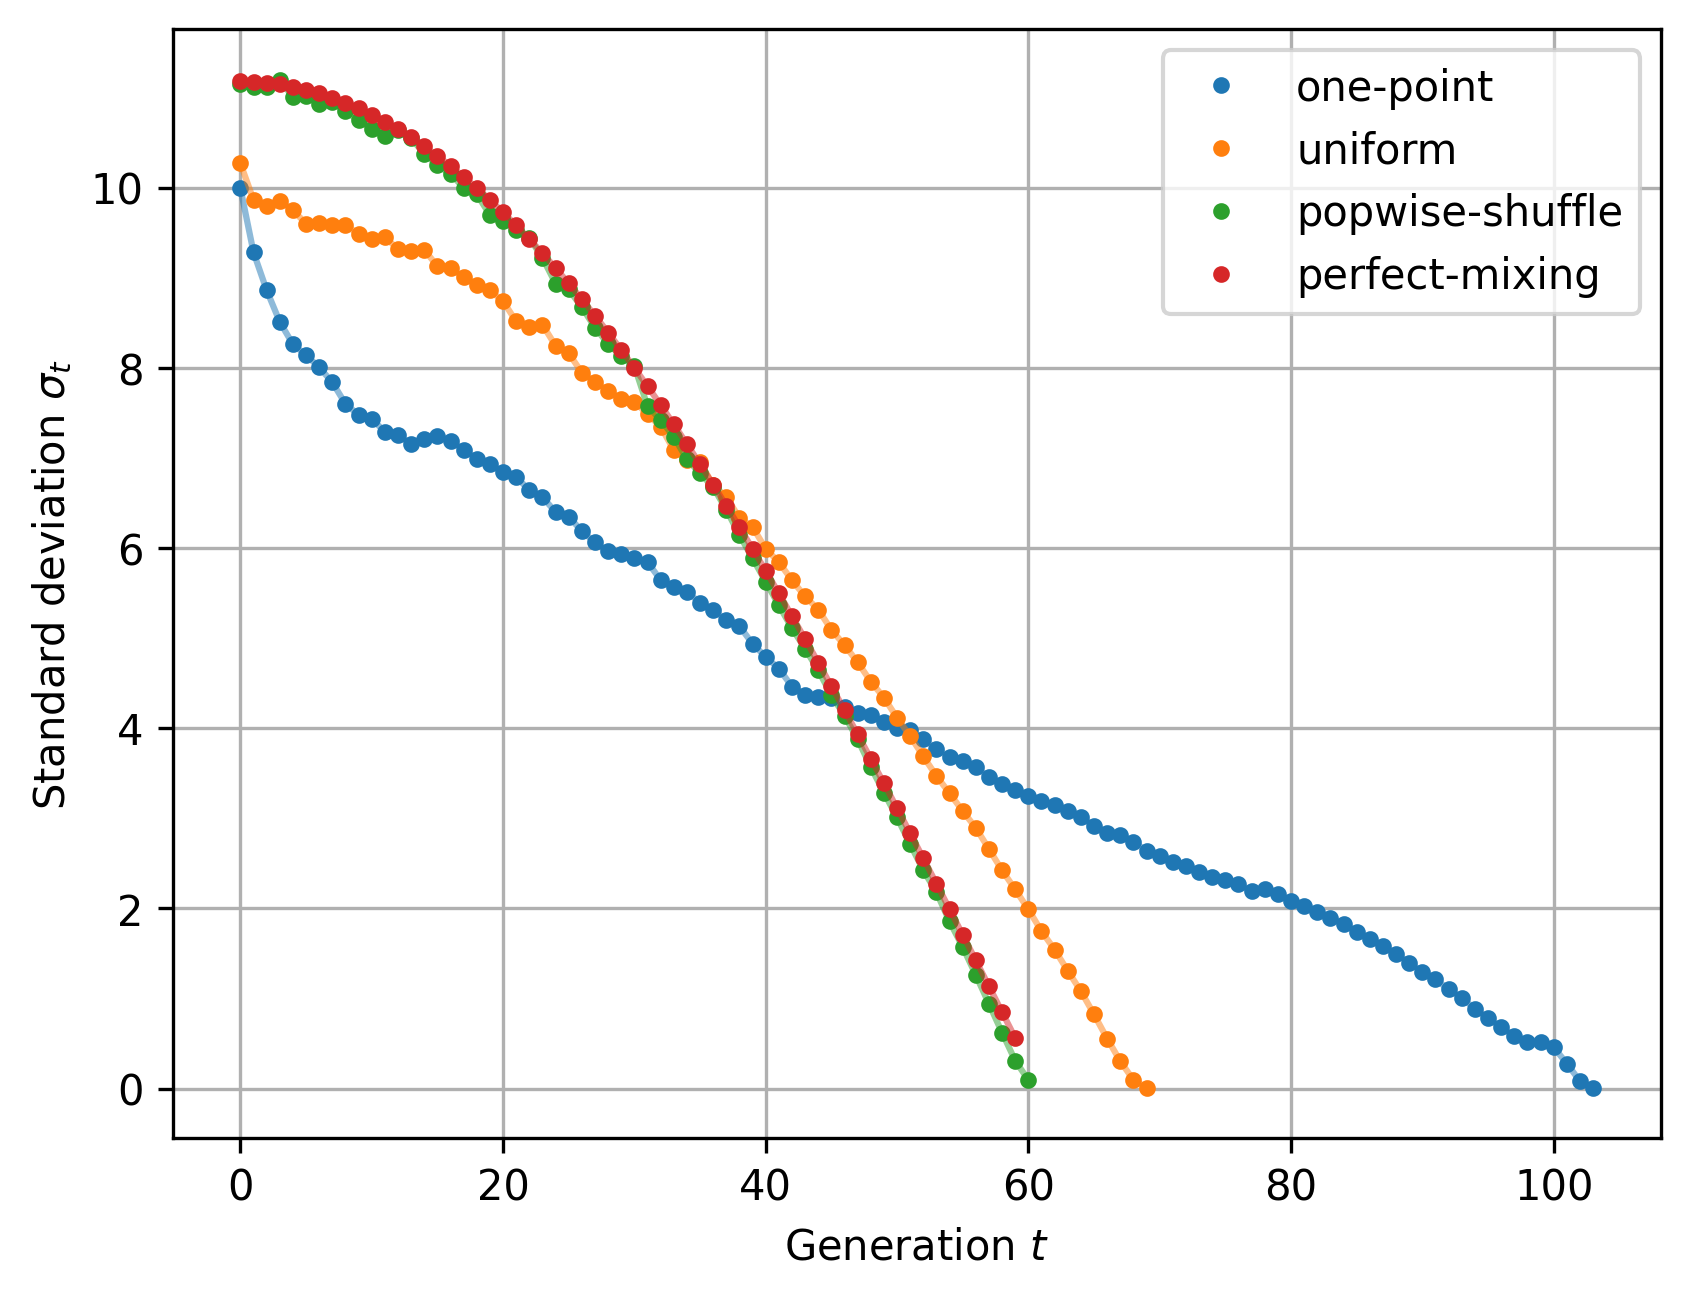
\includegraphics[width=\linewidth]{fig-std_500.png}
                  \caption{$ell=500$}
                  \label{fig:std-500}
            \end{subfigure}
            \caption{Standard deviation of different XO methods}
            \label{fig:std}
      \end{figure}
      
      The proportion of the unitation and the standard deviation of the fitness values with problem size 50, 250, and 500 are 
      shown in Figures~\ref{fig:unitation} and~\ref{fig:std}, respectively.
      In Figure~\ref{fig:unitation}, one-point XO executes more generation to reach the proportion of the unitation 1 than any other XO methods.
      This reflects the curves of the convergence time in Figure~\ref{fig:convergence_time} that the one-point XO has the longest convergence time.
      In Figure~\ref{fig:std}, the standard deviation of the one-point XO and the uniform XO are lower than the perfect mixing and the population-wise shuffling
      at the beginning of the generations. However, the decreasing ratio of the one-point XO and the uniform XO are slower than the perfect mixing and the population-wise shuffling.
      This indicates that the one-point XO and the uniform XO have a lower degree of disruption than the perfect mixing and the population-wise shuffling.
      
      In summary, among the three XO methods, the curve trends of perfect mixing and 
      population-wise shuffling exhibit the highest similarity. Particularly for large problem sizes, 
      the curve trends of perfect mixing and population-wise shuffling nearly coincide, suggesting that 
      population-wise shuffling closely resembles perfect mixing in terms of unitation and standard deviation of fitness values. 
      Therefore, in the OneMax problem executed by SGA, utilizing the XO method with greater disruption 
       leads to shorter convergence times.
      \hfill $\square$

\end{enumerate}




















% \section{Some examples to get started}

% \subsection{How to create Sections and Subsections}

% Simply use the section and subsection commands, as in this example document! With Overleaf, all the formatting and numbering is handled automatically according to the template you've chosen. If you're using the Visual Editor, you can also create new section and subsections via the buttons in the editor toolbar.

% \subsection{How to include Figures}

% First you have to upload the image file from your computer using the upload link in the file-tree menu. Then use the includegraphics command to include it in your document. Use the figure environment and the caption command to add a number and a caption to your figure. See the code for Figure \ref{fig:frog} in this section for an example.

% Note that your figure will automatically be placed in the most appropriate place for it, given the surrounding text and taking into account other figures or tables that may be close by. You can find out more about adding images to your documents in this help article on \href{https://www.overleaf.com/learn/how-to/Including_images_on_Overleaf}{including images on Overleaf}.

% % \begin{figure}
% % \centering
% % \includegraphics[width=0.25\linewidth]{frog.jpg}
% % \caption{\label{fig:frog}This frog was uploaded via the file-tree menu.}
% % \end{figure}

% \subsection{How to add Tables}

% Use the table and tabular environments for basic tables --- see Table~\ref{tab:widgets}, for example. For more information, please see this help article on \href{https://www.overleaf.com/learn/latex/tables}{tables}. 

% \begin{table}
% \centering
% \begin{tabular}{l|r}
% Item & Quantity \\\hline
% Widgets & 42 \\
% Gadgets & 13
% \end{tabular}
% \caption{\label{tab:widgets}An example table.}
% \end{table}

% \subsection{How to add Comments and Track Changes}

% Comments can be added to your project by highlighting some text and clicking ``Add comment'' in the top right of the editor pane. To view existing comments, click on the Review menu in the toolbar above. To reply to a comment, click on the Reply button in the lower right corner of the comment. You can close the Review pane by clicking its name on the toolbar when you're done reviewing for the time being.

% Track changes are available on all our \href{https://www.overleaf.com/user/subscription/plans}{premium plans}, and can be toggled on or off using the option at the top of the Review pane. Track changes allow you to keep track of every change made to the document, along with the person making the change. 

% \subsection{How to add Lists}

% You can make lists with automatic numbering \dots

% \begin{enumerate}
% \item Like this,
% \item and like this.
% \end{enumerate}
% \dots or bullet points \dots
% \begin{itemize}
% \item Like this,
% \item and like this.
% \end{itemize}

% \subsection{How to write Mathematics}

% \LaTeX{} is great at typesetting mathematics. Let $X_1, X_2, \ldots, X_n$ be a sequence of independent and identically distributed random variables with $\text{E}[X_i] = \mu$ and $\text{Var}[X_i] = \sigma^2 < \infty$, and let
% \[S_n = \frac{X_1 + X_2 + \cdots + X_n}{n}
%       = \frac{1}{n}\sum_{i}^{n} X_i\]
% denote their mean. Then as $n$ approaches infinity, the random variables $\sqrt{n}(S_n - \mu)$ converge in distribution to a normal $\mathcal{N}(0, \sigma^2)$.


% \subsection{How to change the margins and paper size}

% Usually the template you're using will have the page margins and paper size set correctly for that use-case. For example, if you're using a journal article template provided by the journal publisher, that template will be formatted according to their requirements. In these cases, it's best not to alter the margins directly.

% If however you're using a more general template, such as this one, and would like to alter the margins, a common way to do so is via the geometry package. You can find the geometry package loaded in the preamble at the top of this example file, and if you'd like to learn more about how to adjust the settings, please visit this help article on \href{https://www.overleaf.com/learn/latex/page_size_and_margins}{page size and margins}.

% \subsection{How to change the document language and spell check settings}

% Overleaf supports many different languages, including multiple different languages within one document. 

% To configure the document language, simply edit the option provided to the babel package in the preamble at the top of this example project. To learn more about the different options, please visit this help article on \href{https://www.overleaf.com/learn/latex/International_language_support}{international language support}.

% To change the spell check language, simply open the Overleaf menu at the top left of the editor window, scroll down to the spell check setting, and adjust accordingly.

% \subsection{How to add Citations and a References List}

% You can simply upload a \verb|.bib| file containing your BibTeX entries, created with a tool such as JabRef. You can then cite entries from it, like this: \cite{greenwade93}. Just remember to specify a bibliography style, as well as the filename of the \verb|.bib|. You can find a \href{https://www.overleaf.com/help/97-how-to-include-a-bibliography-using-bibtex}{video tutorial here} to learn more about BibTeX.

% If you have an \href{https://www.overleaf.com/user/subscription/plans}{upgraded account}, you can also import your Mendeley or Zotero library directly as a \verb|.bib| file, via the upload menu in the file-tree.

% \subsection{Good luck!}

% We hope you find Overleaf useful, and do take a look at our \href{https://www.overleaf.com/learn}{help library} for more tutorials and user guides! Please also let us know if you have any feedback using the Contact Us link at the bottom of the Overleaf menu --- or use the contact form at \url{https://www.overleaf.com/contact}.

% \bibliographystyle{alpha}
% \bibliography{sample}
% \end{CJK*}
\end{document}